
\medskip

Les baleines émettent des sons, de fréquences comprises entre 10~Hz et 10~kHz, qui se
propagent dans l'eau à une vitesse d'environ \np{1500}~m/s.

L'étude des chants des baleines a pour but d'élucider leur possible signification ; sélection du partenaire sexuel et communication sociale sont des hypothèses envisagées.

\medskip

\begin{enumerate}
\item Convertir la vitesse de propagation de ces sons en km/h.
\item Deux groupes de baleines situées au large de l'Alaska communiquent entre eux.
	\begin{enumerate}
		\item Calculer la distance séparant les deux groupes de baleines. 
		
\emph{Vous donnerez le résultat arrondi à $50$km près.}

\begin{center}
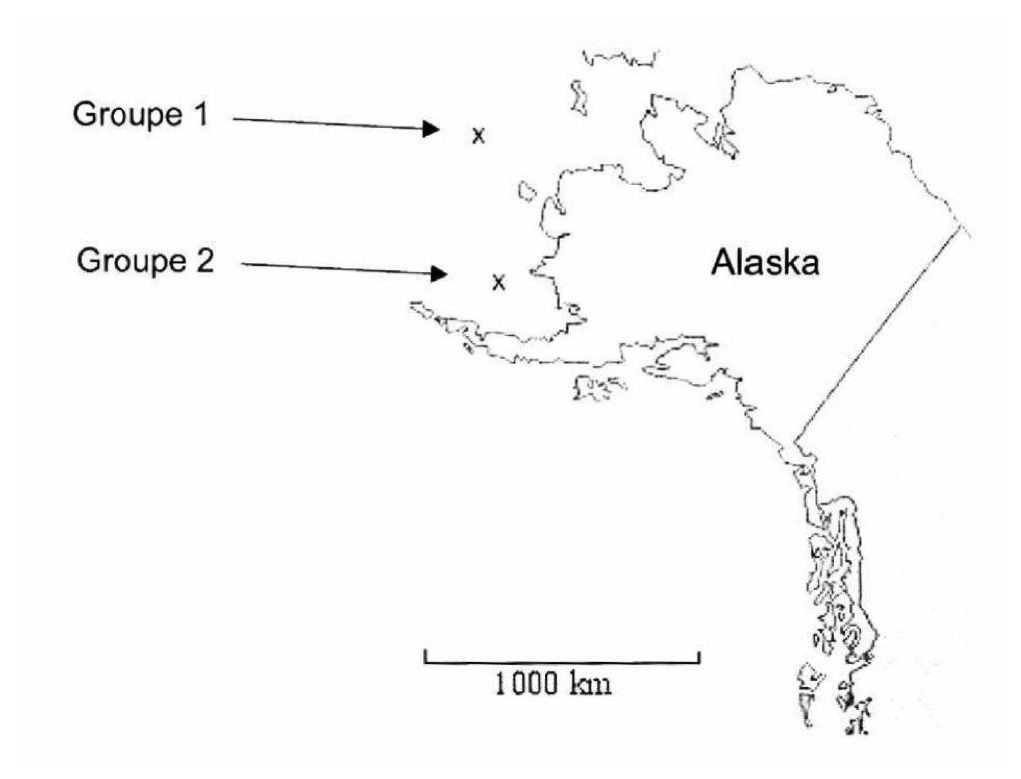
\includegraphics[width=9cm]{Alaska}
\end{center}

		\item Combien de temps met une onde sonore émise par une baleine du groupe 1 pour
parvenir aux baleines du groupe 2 ? 

\emph{Vous donnerez le résultat arrondi à la minute.}
 	\end{enumerate}
\item  Le dessin ci-dessous donne une idée de la taille d'une baleine bleue par rapport à celle d'un homme.
	
En considérant que le plongeur sur l'image a une taille égale à $1,75$~m, calculer la taille approximative de la baleine représentée ci-dessous. 
	
\emph{Vous donnerez le résultat arrondi au mètre près.}

\emph{La démarche et les traces de recherche seront valorisées et prises en compte dans la notation.}

\begin{center}

\includegraphics[width=12cm]{baleine}
\end{center}
\end{enumerate}

\bigskip

